\documentclass[14pt]{extbook}
\usepackage{multicol, enumerate, enumitem, hyperref, color, soul, setspace, parskip, fancyhdr} %General Packages
\usepackage{amssymb, amsthm, amsmath, latexsym, units, mathtools} %Math Packages
\everymath{\displaystyle} %All math in Display Style
% Packages with additional options
\usepackage[headsep=0.5cm,headheight=12pt, left=1 in,right= 1 in,top= 1 in,bottom= 1 in]{geometry}
\usepackage[usenames,dvipsnames]{xcolor}
\usepackage{dashrule}  % Package to use the command below to create lines between items
\newcommand{\litem}[1]{\item#1\hspace*{-1cm}\rule{\textwidth}{0.4pt}}
\pagestyle{fancy}
\lhead{Makeup Progress Quiz 2}
\chead{}
\rhead{Version A}
\lfoot{5763-3522}
\cfoot{}
\rfoot{Spring 2021}
\begin{document}

\begin{enumerate}
\litem{
Graph the equation below.\[ f(x) = -(x-4)^2 - 12 \]\begin{enumerate}[label=\Alph*.]
\begin{multicols}{2}\item 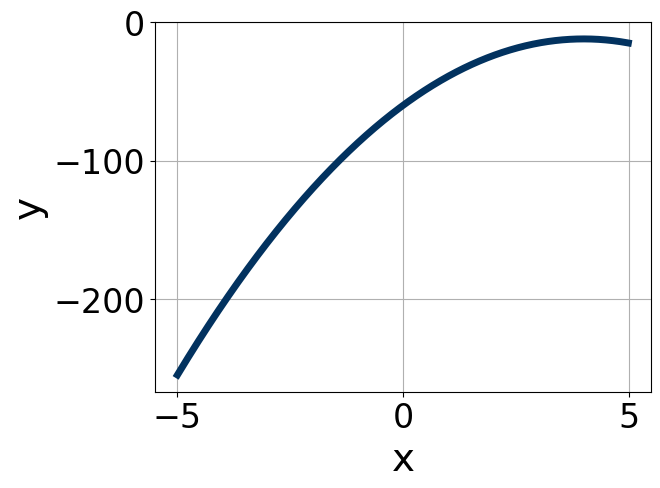
\includegraphics[width = 0.3\textwidth]{../Figures/quadraticEquationToGraphAA.png}\item 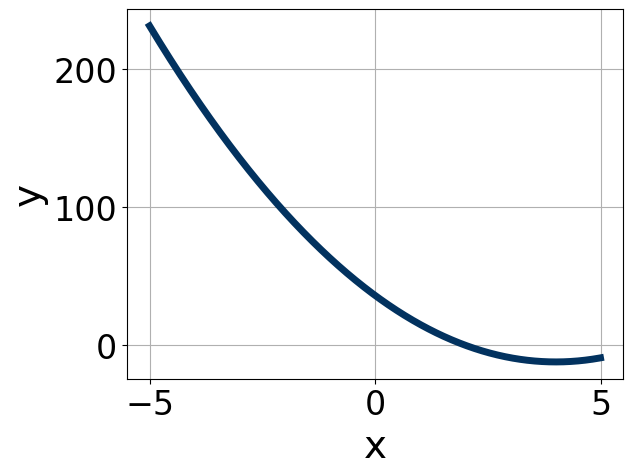
\includegraphics[width = 0.3\textwidth]{../Figures/quadraticEquationToGraphBA.png}\item 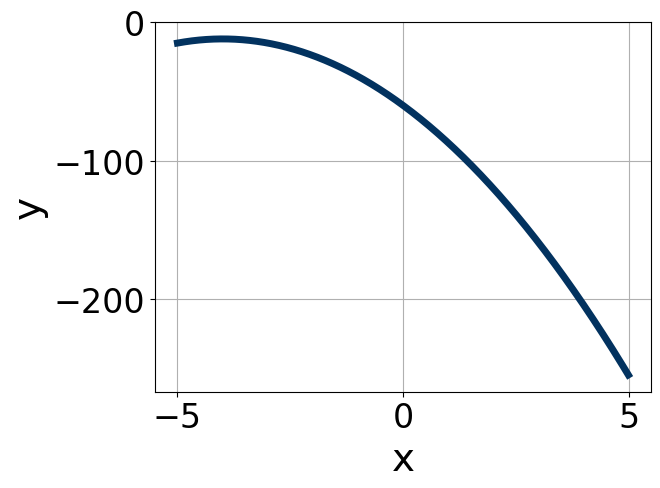
\includegraphics[width = 0.3\textwidth]{../Figures/quadraticEquationToGraphCA.png}\item 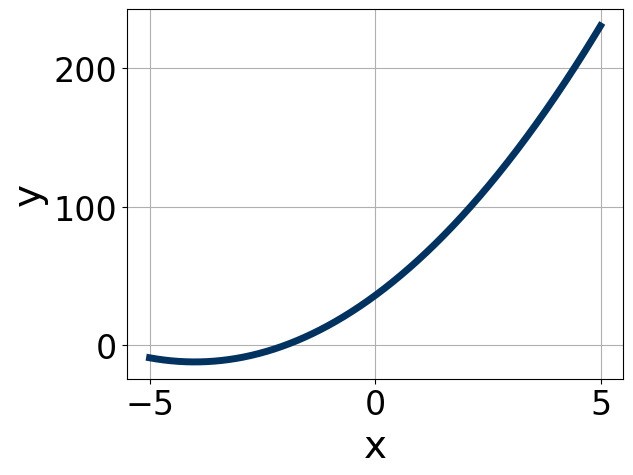
\includegraphics[width = 0.3\textwidth]{../Figures/quadraticEquationToGraphDA.png}\end{multicols}\item None of the above.
\end{enumerate} }
\litem{
Write the equation of the graph presented below in the form $f(x)=ax^2+bx+c$, assuming  $a=1$ or $a=-1$. Then, choose the intervals that $a, b,$ and $c$ belong to.
\begin{center}
    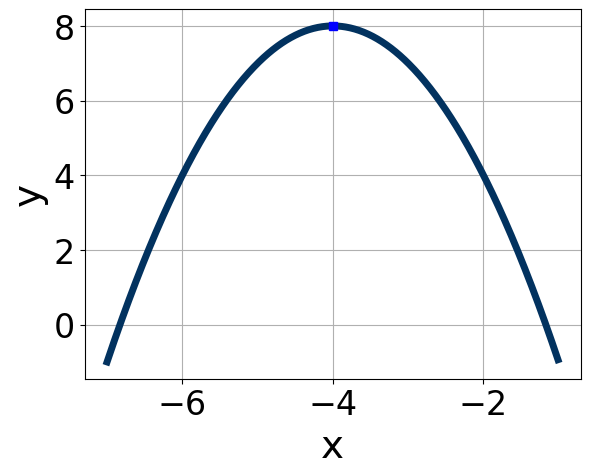
\includegraphics[width=0.5\textwidth]{../Figures/quadraticGraphToEquationA.png}
\end{center}
\begin{enumerate}[label=\Alph*.]
\item \( a \in [-2.4, -0.8], \hspace*{5mm} b \in [-8, -5], \text{ and } \hspace*{5mm} c \in [-9, -7] \)
\item \( a \in [-2.4, -0.8], \hspace*{5mm} b \in [8, 13], \text{ and } \hspace*{5mm} c \in [-24, -22] \)
\item \( a \in [0, 1.9], \hspace*{5mm} b \in [8, 13], \text{ and } \hspace*{5mm} c \in [23, 25] \)
\item \( a \in [0, 1.9], \hspace*{5mm} b \in [-8, -5], \text{ and } \hspace*{5mm} c \in [23, 25] \)
\item \( a \in [-2.4, -0.8], \hspace*{5mm} b \in [8, 13], \text{ and } \hspace*{5mm} c \in [-9, -7] \)

\end{enumerate} }
\litem{
Solve the quadratic equation below. Then, choose the intervals that the solutions $x_1$ and $x_2$ belong to, with $x_1 \leq x_2$.\[ 25x^{2} +10 x -24 = 0 \]\begin{enumerate}[label=\Alph*.]
\item \( x_1 \in [-0.99, 1.03] \text{ and } x_2 \in [1.6, 1.85] \)
\item \( x_1 \in [-1.26, -1.05] \text{ and } x_2 \in [0.59, 0.85] \)
\item \( x_1 \in [-30.21, -29.25] \text{ and } x_2 \in [19.66, 20.07] \)
\item \( x_1 \in [-6.46, -5.81] \text{ and } x_2 \in [0.09, 0.27] \)
\item \( x_1 \in [-3.59, -1.91] \text{ and } x_2 \in [0.23, 0.44] \)

\end{enumerate} }
\litem{
Solve the quadratic equation below. Then, choose the intervals that the solutions belong to, with $x_1 \leq x_2$ (if they exist).\[ -19x^{2} -13 x + 8 = 0 \]\begin{enumerate}[label=\Alph*.]
\item \( x_1 \in [-0.59, -0.36] \text{ and } x_2 \in [0.8, 1.09] \)
\item \( x_1 \in [-8.09, -6.62] \text{ and } x_2 \in [19.52, 21.03] \)
\item \( x_1 \in [-2.28, -0.62] \text{ and } x_2 \in [-0.05, 0.79] \)
\item \( x_1 \in [-28.5, -27.22] \text{ and } x_2 \in [27.25, 27.76] \)
\item \( \text{There are no Real solutions.} \)

\end{enumerate} }
\litem{
Graph the equation below.\[ f(x) = (x-4)^2 + 19 \]\begin{enumerate}[label=\Alph*.]
\begin{multicols}{2}\item 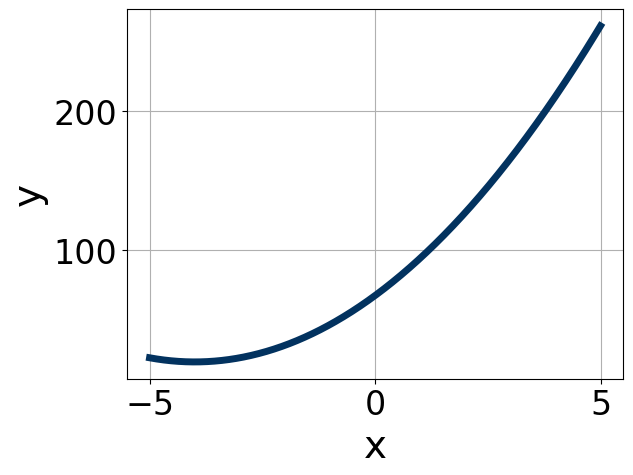
\includegraphics[width = 0.3\textwidth]{../Figures/quadraticEquationToGraphCopyAA.png}\item 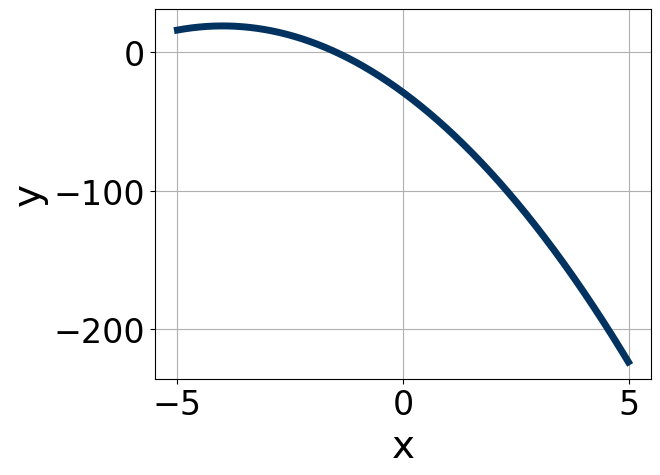
\includegraphics[width = 0.3\textwidth]{../Figures/quadraticEquationToGraphCopyBA.png}\item 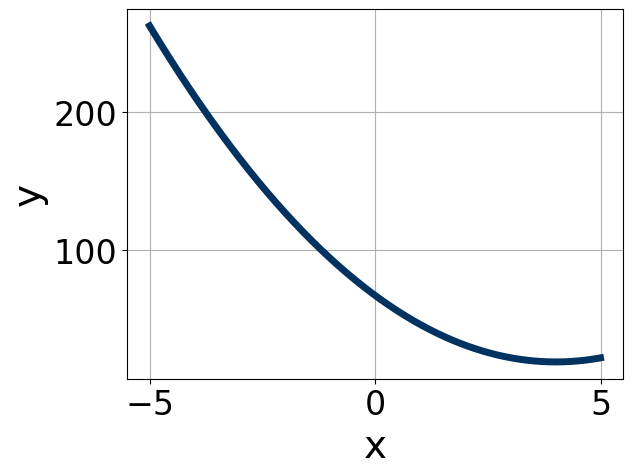
\includegraphics[width = 0.3\textwidth]{../Figures/quadraticEquationToGraphCopyCA.png}\item 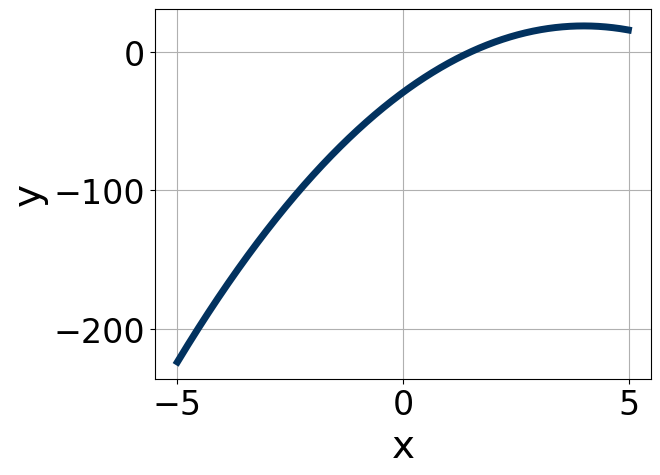
\includegraphics[width = 0.3\textwidth]{../Figures/quadraticEquationToGraphCopyDA.png}\end{multicols}\item None of the above.
\end{enumerate} }
\litem{
Factor the quadratic below. Then, choose the intervals that contain the constants in the form $(ax+b)(cx+d); b \leq d.$\[ 36x^{2} -60 x + 25 \]\begin{enumerate}[label=\Alph*.]
\item \( a \in [1.3, 3.4], \hspace*{5mm} b \in [-8, -4], \hspace*{5mm} c \in [11.92, 12.96], \text{ and } \hspace*{5mm} d \in [-6, -4] \)
\item \( a \in [11.5, 12.3], \hspace*{5mm} b \in [-8, -4], \hspace*{5mm} c \in [2.18, 4.16], \text{ and } \hspace*{5mm} d \in [-6, -4] \)
\item \( a \in [5.1, 6.1], \hspace*{5mm} b \in [-8, -4], \hspace*{5mm} c \in [5.73, 6.44], \text{ and } \hspace*{5mm} d \in [-6, -4] \)
\item \( a \in [-1.3, 2.4], \hspace*{5mm} b \in [-30, -25], \hspace*{5mm} c \in [0.43, 1.66], \text{ and } \hspace*{5mm} d \in [-36, -25] \)
\item \( \text{None of the above.} \)

\end{enumerate} }
\litem{
Write the equation of the graph presented below in the form $f(x)=ax^2+bx+c$, assuming  $a=1$ or $a=-1$. Then, choose the intervals that $a, b,$ and $c$ belong to.
\begin{center}
    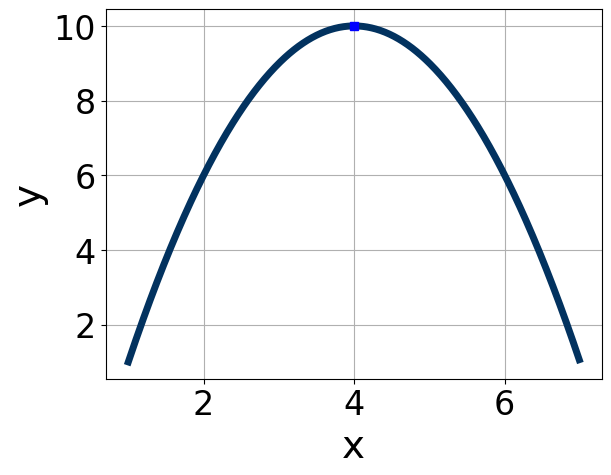
\includegraphics[width=0.5\textwidth]{../Figures/quadraticGraphToEquationCopyA.png}
\end{center}
\begin{enumerate}[label=\Alph*.]
\item \( a \in [0, 4], \hspace*{5mm} b \in [5, 13], \text{ and } \hspace*{5mm} c \in [24, 29] \)
\item \( a \in [-3, 0], \hspace*{5mm} b \in [-10, -3], \text{ and } \hspace*{5mm} c \in [-8, -4] \)
\item \( a \in [-3, 0], \hspace*{5mm} b \in [5, 13], \text{ and } \hspace*{5mm} c \in [-8, -4] \)
\item \( a \in [0, 4], \hspace*{5mm} b \in [-10, -3], \text{ and } \hspace*{5mm} c \in [24, 29] \)
\item \( a \in [-3, 0], \hspace*{5mm} b \in [-10, -3], \text{ and } \hspace*{5mm} c \in [-29, -25] \)

\end{enumerate} }
\litem{
Factor the quadratic below. Then, choose the intervals that contain the constants in the form $(ax+b)(cx+d); b \leq d.$\[ 54x^{2} -57 x + 10 \]\begin{enumerate}[label=\Alph*.]
\item \( a \in [4.7, 7.43], \hspace*{5mm} b \in [-6, -4], \hspace*{5mm} c \in [6.4, 9.9], \text{ and } \hspace*{5mm} d \in [-4, -1] \)
\item \( a \in [11.56, 13.06], \hspace*{5mm} b \in [-6, -4], \hspace*{5mm} c \in [2, 6], \text{ and } \hspace*{5mm} d \in [-4, -1] \)
\item \( a \in [1.76, 2.81], \hspace*{5mm} b \in [-6, -4], \hspace*{5mm} c \in [25.8, 29.8], \text{ and } \hspace*{5mm} d \in [-4, -1] \)
\item \( a \in [-0.38, 1.28], \hspace*{5mm} b \in [-45, -41], \hspace*{5mm} c \in [-3.3, 3.1], \text{ and } \hspace*{5mm} d \in [-15, -10] \)
\item \( \text{None of the above.} \)

\end{enumerate} }
\litem{
Solve the quadratic equation below. Then, choose the intervals that the solutions belong to, with $x_1 \leq x_2$ (if they exist).\[ -13x^{2} -13 x + 5 = 0 \]\begin{enumerate}[label=\Alph*.]
\item \( x_1 \in [-2.2, -0.3] \text{ and } x_2 \in [-0.4, 0.8] \)
\item \( x_1 \in [-22.1, -19.4] \text{ and } x_2 \in [18.9, 21.4] \)
\item \( x_1 \in [-1, 0.8] \text{ and } x_2 \in [0.8, 3.5] \)
\item \( x_1 \in [-4.7, -2.9] \text{ and } x_2 \in [16.7, 19.1] \)
\item \( \text{There are no Real solutions.} \)

\end{enumerate} }
\litem{
Solve the quadratic equation below. Then, choose the intervals that the solutions $x_1$ and $x_2$ belong to, with $x_1 \leq x_2$.\[ 15x^{2} -8 x -16 = 0 \]\begin{enumerate}[label=\Alph*.]
\item \( x_1 \in [-0.53, -0.26] \text{ and } x_2 \in [2.52, 2.91] \)
\item \( x_1 \in [-1.86, -1.56] \text{ and } x_2 \in [0.29, 0.9] \)
\item \( x_1 \in [-0.85, -0.47] \text{ and } x_2 \in [0.89, 1.7] \)
\item \( x_1 \in [-4.15, -3.77] \text{ and } x_2 \in [0.23, 0.51] \)
\item \( x_1 \in [-12.26, -11.69] \text{ and } x_2 \in [19.56, 20.04] \)

\end{enumerate} }
\end{enumerate}

\end{document}